L'applicativo, oltre a seguire un design MVC, per la separazione dei componenti, implementa anche un pattern di comunicazione ad eventi, meglio conosciuto come \textit{pattern observer-delegate}. 
In sostanza, ogni componente che necessita di una certa tipologia di informazioni, si mette in ascolto, registrandosi ad un "servizio" offerto nel nostro caso dal \textit{DataDispatcherSingleton}, il quale va a salvarsi al suo interno un gruppo di riferimenti (delegati) che dovrà poi andare a notificare nel momento in cui risulteranno essere presenti nuove informazioni a cui gli observers stessi sono interessati.
Come si può ben capire si tratta quindi di un pattern molto vicino alla struttura \textit{Publish-Subscribe}, con il quale si definisce una dipendenza uno a molti fra gli oggetti: in sostanza abbiano un oggetto che viene \textit{osservato} e tanti oggetti che \textit{osservano} i cambiamenti di quest'ultimo, come si può vedere nella struttura generica rappresentata in figura ~\ref{fig:ObserverStructure}:

\begin{figure}[h]
	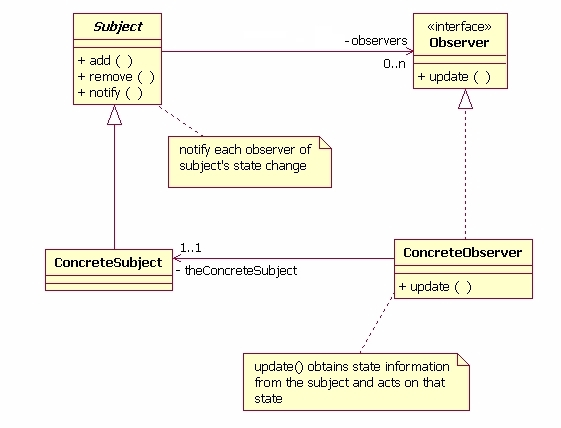
\includegraphics[width=\textwidth]{Immagini/Observer/ObserverTheory.jpg}
	\caption{Struttura generica pattern observer}
	\label{fig:ObserverStructure}
\end{figure}

Questa struttura è stata riprodotta anche nel nostro applicativo, dove possiamo vedere la presenza di alcune struttura caratteristiche di questo pattern: abbiamo una funzionalità di \textit{register}, che, a seconda di quale observer chiama questa funziona, lo pone nel vettore specifico (figura ~\ref{fig:RegisterFunction}). Per evitare di avere dipendenze cicliche, o comunque per mantenere una certa pulizia nei riferimenti tra classi, p necessario che ogni observer, nel momento in cui non necessita più di una certa tipologie di informazioni, vada a deregistrarsi: questa operazione consiste nell'andare a togliere il qualsiasi riferimento all'oggetto in esame dall'interno del \textit{DataDispatcherSingleton}, come fatto in figura ~\ref{fig:UnregisterFunction}.

\begin{figure}[h]
	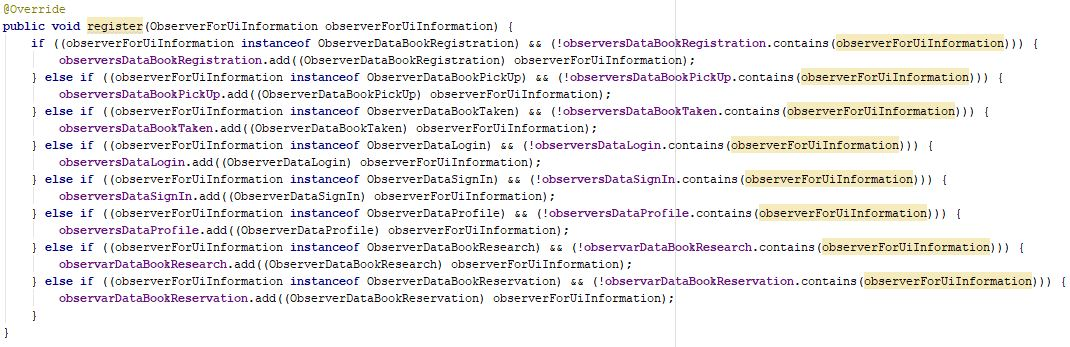
\includegraphics[width=\textwidth]{Immagini/Observer/RegisterToDispatcherData.JPG}
	\caption{Register function}
	\label{fig:RegisterFunction}
\end{figure}

\begin{figure}[h]
	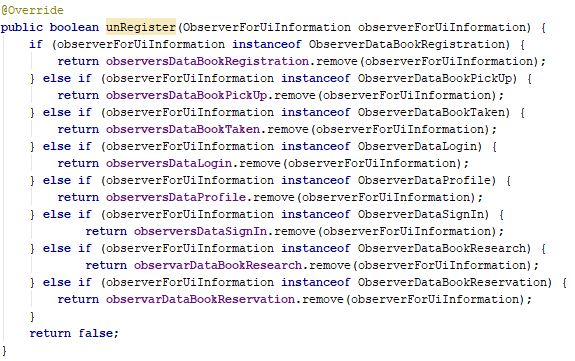
\includegraphics[width=\textwidth]{Immagini/Observer/UnregisterFromDispatcherData.JPG}
	\caption{Unregister function}
	\label{fig:UnregisterFunction}
\end{figure}

Per quanto riguarda invece la parte di \textit{notifica}, abbiamo introdotto un pattern ad eventi custom, che permettesse così di mantenere separata l'implementazione delle informazioni ottenuto da ogni singolo fragment, come si vede nella figura ~\ref{fig:ObserverForUiInformation}.
\begin{figure}[h]
	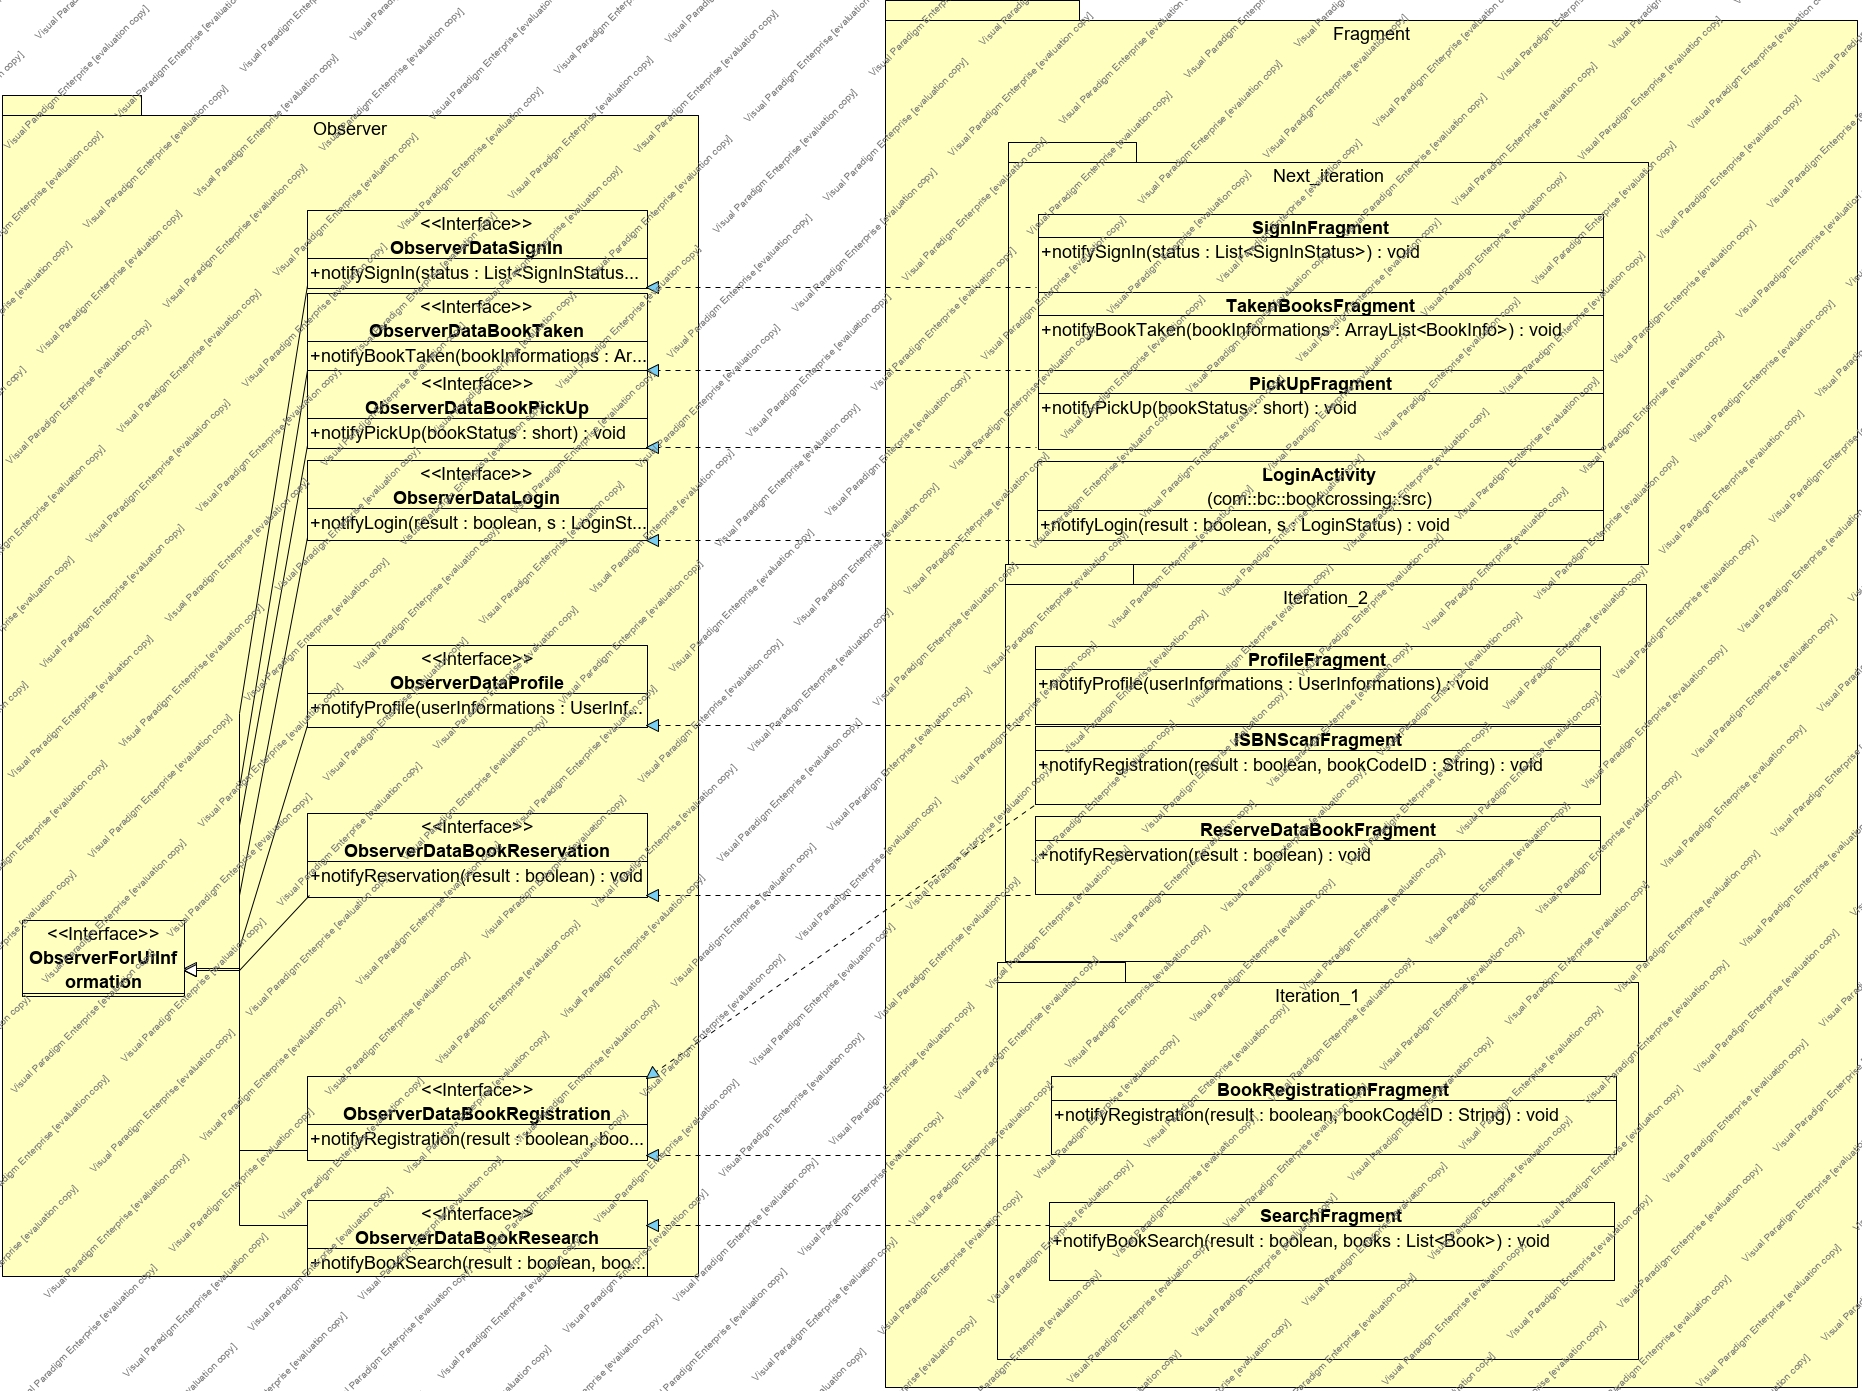
\includegraphics[width=\textwidth]{Immagini/ObserverForUIInformation}
	\caption{Interfaccie per la ricezione degli eventi}
	\label{fig:ObserverForUiInformation}
\end{figure}

Ogni singola interfaccia implementa un'interfaccia comune: questa scelta è stata adotta per rendere del tutto generico il tipo di observer che va a registrarsi per gli eventi forniti dal delegate: infatti, come si può vedere nell'interfaccia \textit{DelegateSendData} (figura ~\ref{fig:DataDispatcher}), chi è interessato ad ottenere informazioni specifiche, si registra come un oggeto di tipo \textit{ObserverForUiInformation}; sarà poi compito del delegate fornire le corrette informazioni, richiamando le corrette funzioni di notifica, le quali sono direttamente implementata all'interno di ogni singola interfaccia concreta.

\begin{figure}[h]
	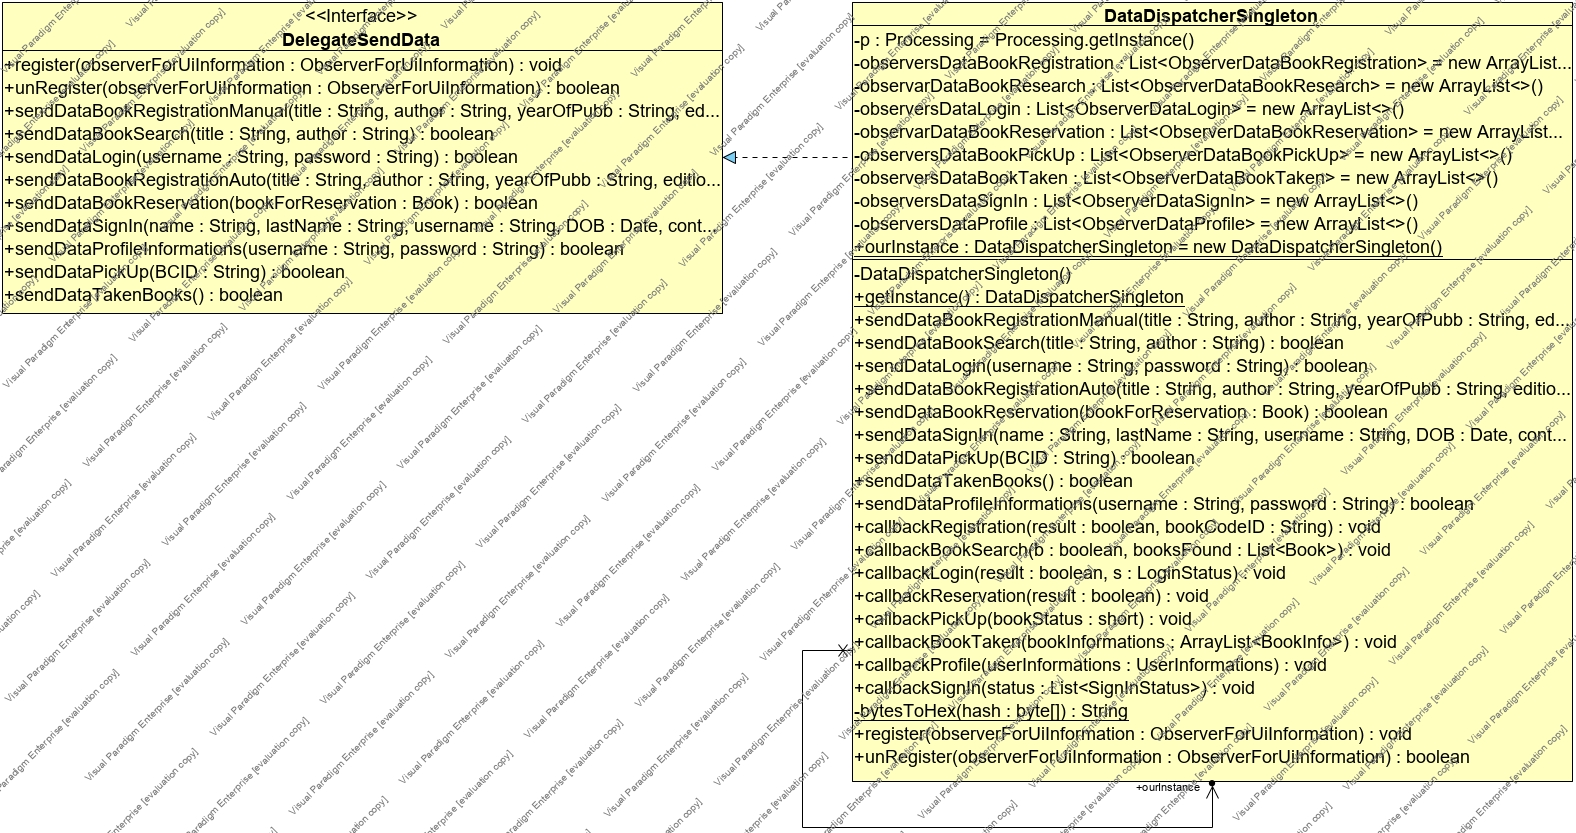
\includegraphics[width=\textwidth]{Immagini/ClassDiagramDispatcherDelegate}
	\caption{Struttura del componente \textit{DataDispatcher}}
	\label{fig:DataDispatcher}
\end{figure}

Si può quindi vedere che, nella struttura predisposta, il \textit{DataDispatcher} lavora come se fosse un \textbf{repository}, ovvero un contenitore di informazioni, che fornisce a tutti gli elementi che si registrano e che ne richiedono la ricezione.

Questi elementi, allo stadio implementativo attuale, sono rappresentati da tutti i fragment, che necessitano di ricevere/inviare informazioni per soddisfare l'interazione con l'utente: come si può notare nelle figure ~\ref{fig:LoginFragment}-~\ref{fig:LoginFragment}-~\ref{fig:BookRegistrationFragment}-~\ref{fig:PickUpFragment}-~\ref{fig:ProfileFragment}-~\ref{fig:SignInFragment}-~\ref{fig:TakenBooksFragment}, ogni singolo fragment è predisposto per ricevere le informazioni di cui ha bisogno, tramite la chiamata delle callback da parte del dispatcher stesso.


\begin{figure}[h!]
	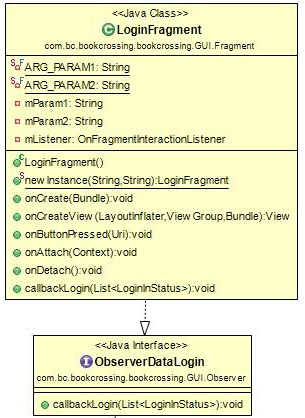
\includegraphics[width=0.5\textwidth]{Immagini/LoginFragment}
	\caption{Struttura del componente \textit{LoginFragment}}
	\label{fig:LoginFragment}
\end{figure}

\begin{figure}[h!]
	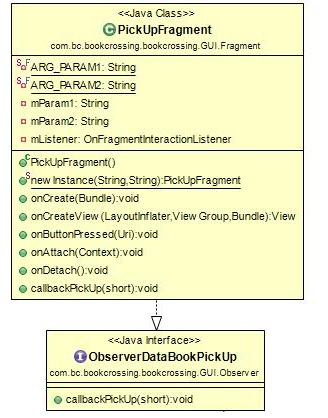
\includegraphics[width=0.5\textwidth]{Immagini/PickUpFragment}
	\caption{Struttura del componente \textit{PickUpFragment}}
	\label{fig:PickUpFragment}
\end{figure}

\begin{figure}[h!]
	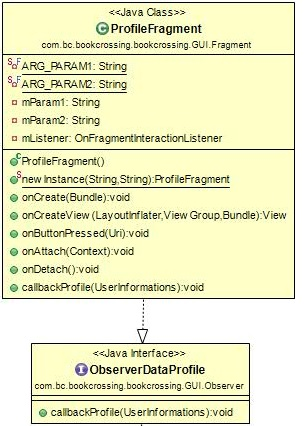
\includegraphics[width=0.5\textwidth]{Immagini/ProfileFragment}
	\caption{Struttura del componente \textit{ProfileFragment}}
	\label{fig:ProfileFragment}
\end{figure}

\begin{figure}[h!]
	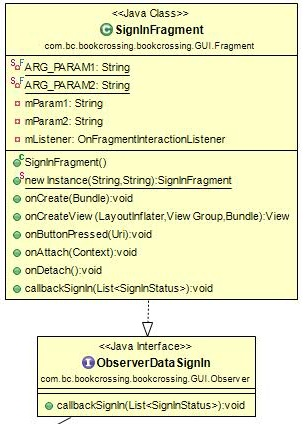
\includegraphics[width=0.5\textwidth]{Immagini/SignInFragment}
	\caption{Struttura del componente \textit{SignInFragment}}
	\label{fig:SignInFragment}
\end{figure}

\begin{figure}[h!]
	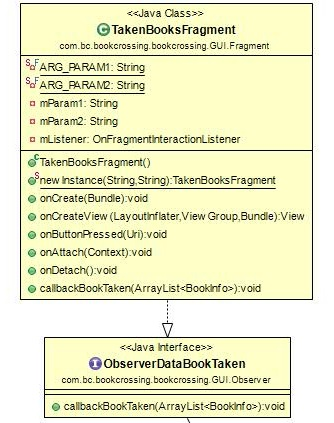
\includegraphics[width=0.5\textwidth]{Immagini/TakenBooksFragment}
	\caption{Struttura del componente \textit{TakenBooksFragment}}
	\label{fig:TakenBooksFragment}
\end{figure}

\begin{figure}[h!]
	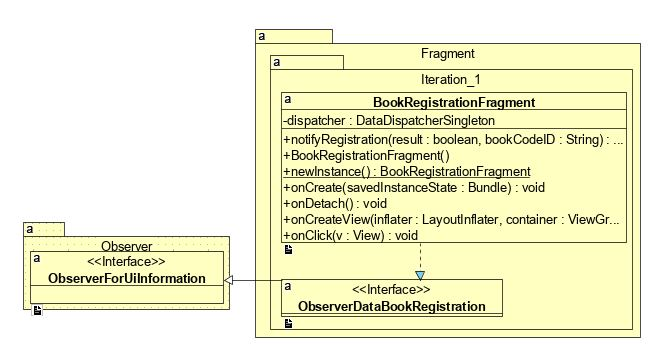
\includegraphics[width=0.5\textwidth]{Immagini/BookRegistrationFragment}
	\caption{Struttura del componente \textit{BookRegistrationFragment}}
	\label{fig:BookRegistrationFragment}
\end{figure}
